\section{Existing Solutions Sufficient?}
\label{sec:existing}
In this section, we explore whether existing network designs can meet the application-level requirements from the network (\S\ref{sec:requirements}), in terms of end-to-end network latency, for the workloads from \S\ref{sec:workloads}. We first describe the methodology in \S\ref{ssec:ssmethod}. We then evaluate the network-level performance for the workloads (\S\ref{ssec:nlp}) for several existing network designs. Finally, we use the results for network-level performance to evaluate the application-level performance (\S\ref{ssec:alp}) in \dis using existing network designs. 

%
\subsection{Methodology}
\label{ssec:ssmethod}
We explore the sufficiency of existing network-layer solutions for \dis in two steps. First, we take the flows generated from \S\ref{sec:workloads} and simulate the network-layer performance (flow completion time) for these flows. We then return to our emulator, take the respective flow completion time for flows, and inject the respective latencies using SIT, as described in \S\ref{sec:requirements}, thus allowing us to evaluate the effect on application level performance. 

%
\begin{figure*}
  \centering
    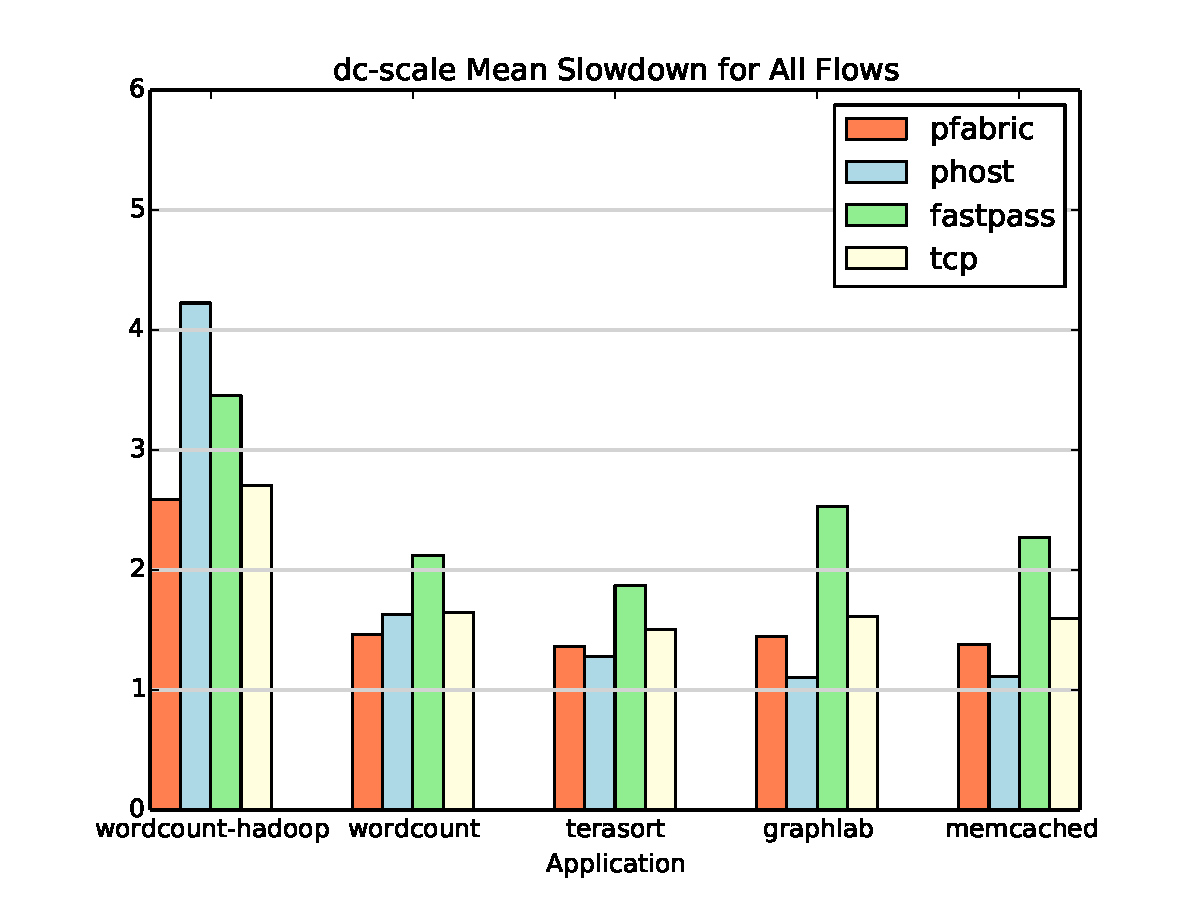
\includegraphics[width = 2in]{img/fig12_dc-scale_slowdowns} 
    \subfigure{
    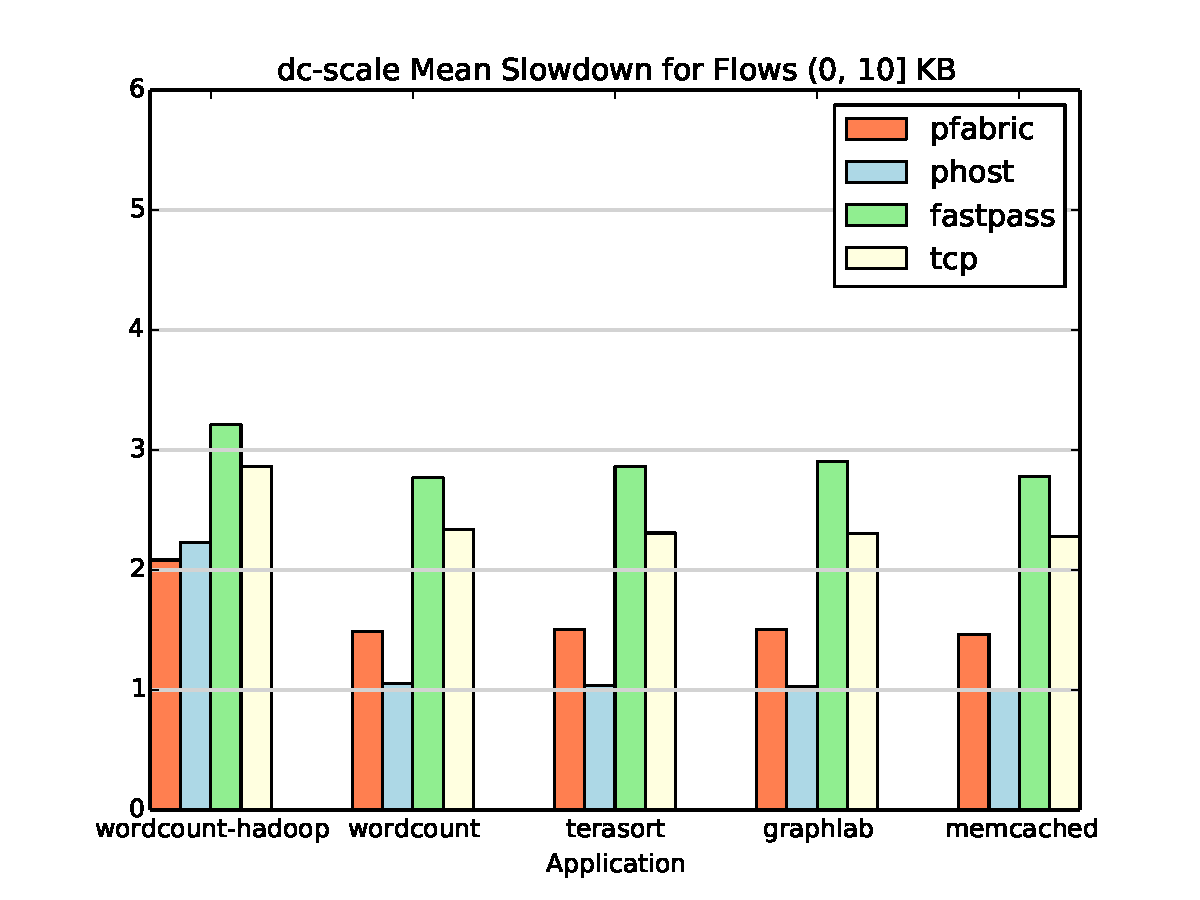
\includegraphics[width=2in]{img/fig12_dc-scale_slowdowns_small}
    }
    \subfigure{
    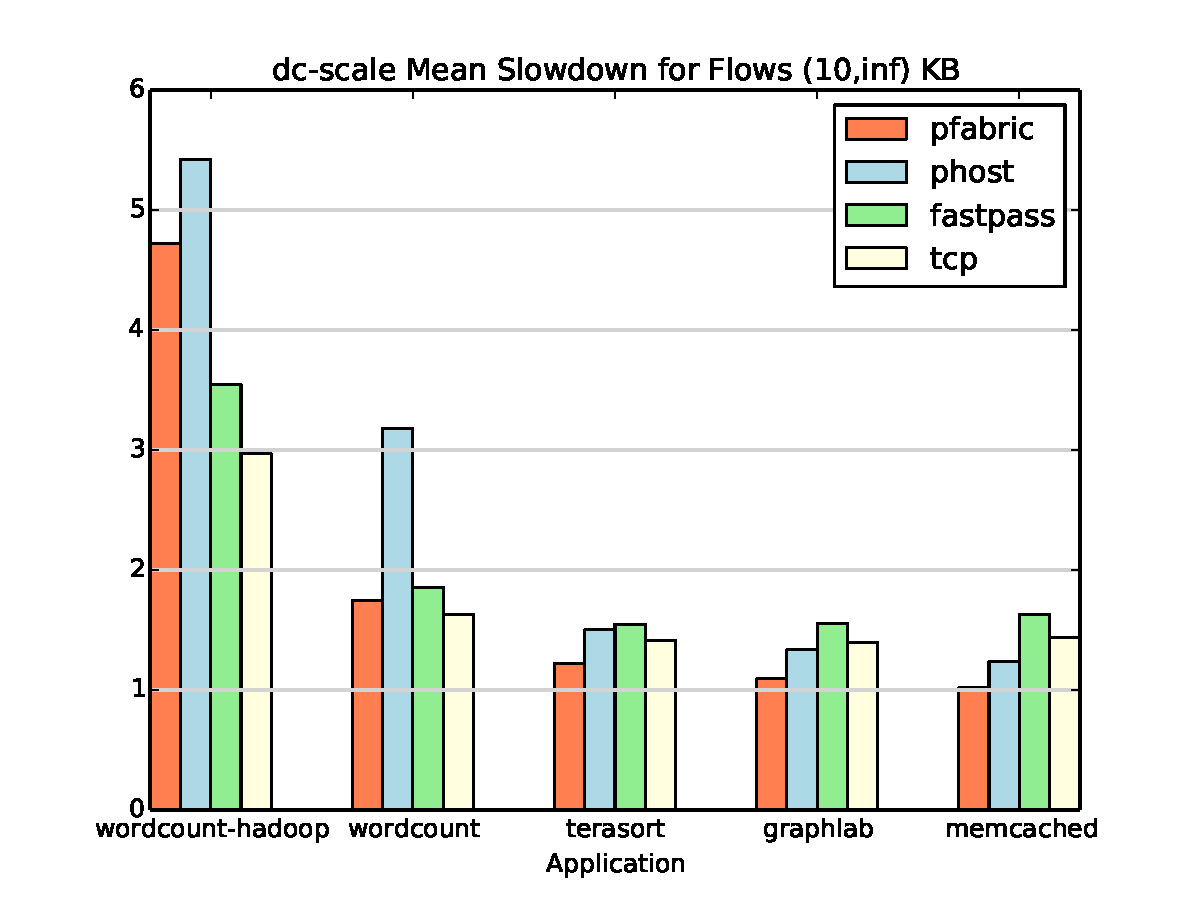
\includegraphics[width=2in]{img/fig12_dc-scale_slowdowns_big}
    }
  \caption{\small{The mean slowdown for pFabric, pHost, fastpass, and TCP for each of the five applications at datacenter-scale: (left) overall; (center) short flows only; (right) long flows.}}
  \label{fig:phostp-ds}
\end{figure*}
%

%
\begin{figure*}
  \centering
    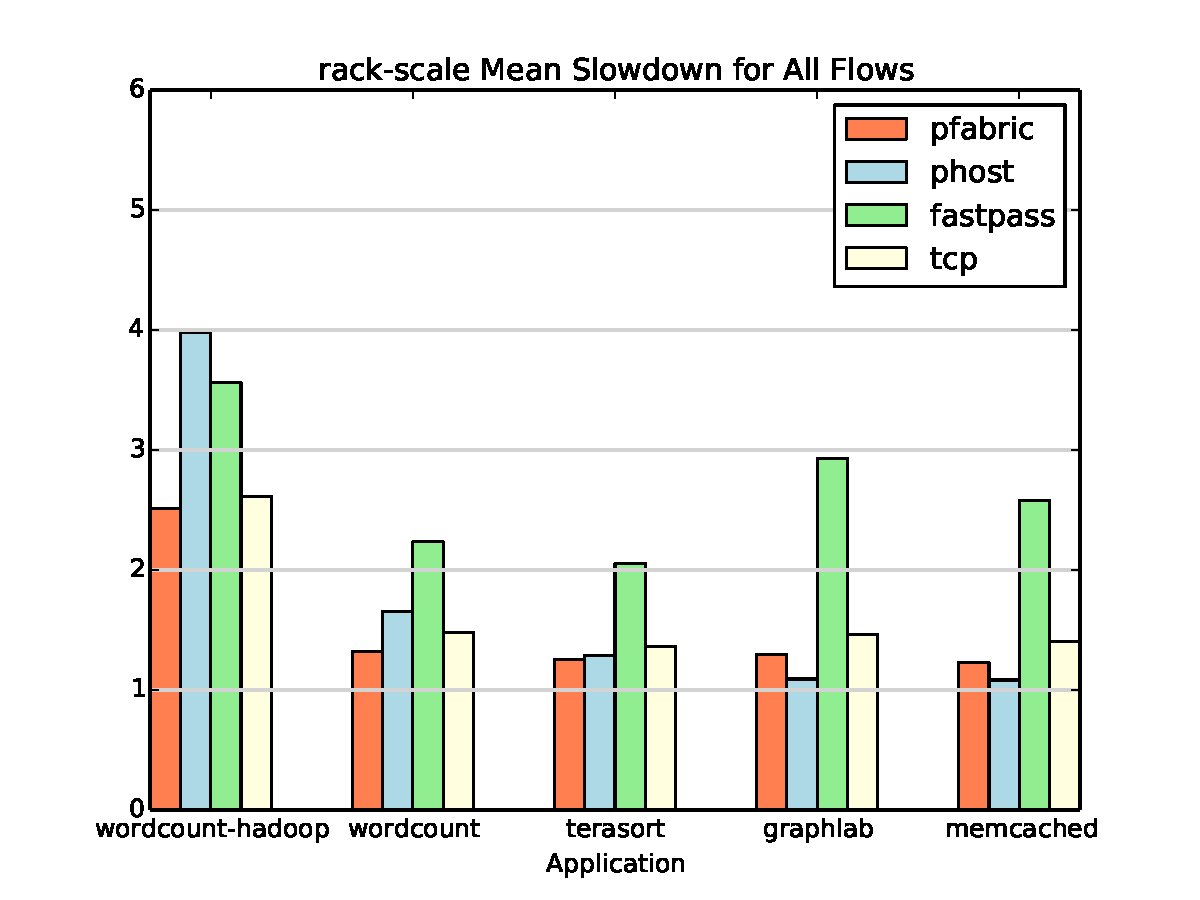
\includegraphics[width = 2in]{img/fig12_rack-scale_slowdowns} 
    \subfigure{
    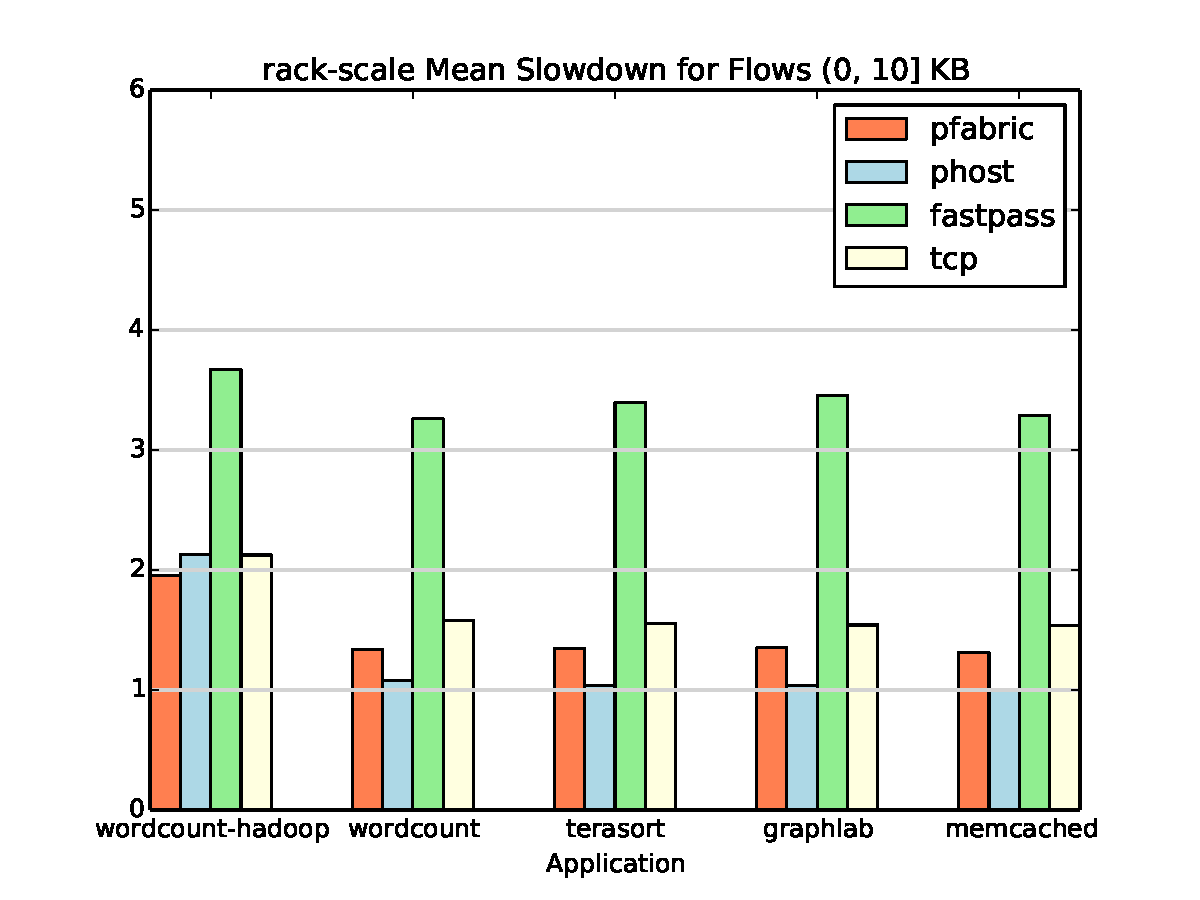
\includegraphics[width=2in]{img/fig12_rack-scale_slowdowns_small}
    }
    \subfigure{
    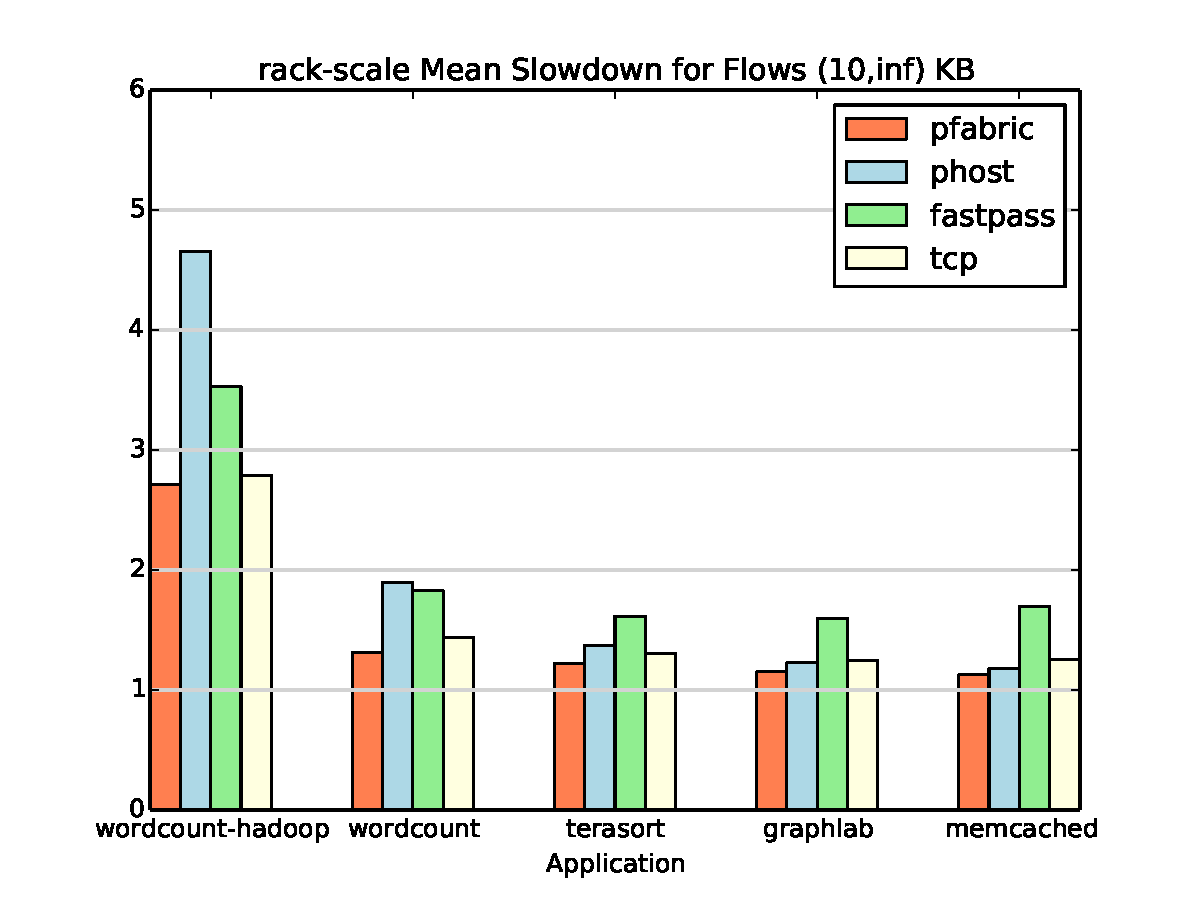
\includegraphics[width=2in]{img/fig12_rack-scale_slowdowns_big}
    }
  \caption{\small{The mean slowdown for pFabric, pHost, fastpass, and TCP for each of the five applications at rack-scale: (left) overall; (center) short flows only; (right) long flows.}}
  \label{fig:phostp-rs}
\end{figure*}
%
For all the simulations in this section, we use the setup from prior work in datacenter transport simulation~\cite{pfabric, phost}. In particular, we simulate a $144$-node full bisection bandwidth fat-tree topology with $40$Gbps access link capacity, $0.2$us of latency per hop, and $36$KB buffers per port. We evaluate the following four protocols:


\begin{enumerate}
\item \paragraphb{pFabric} pFabric~\cite{pfabric} uses priority queues in the network for scheduling and congestion control, prioritizing flows with a smaller remaining flow size. We set pFabric to have an initial congestion window of 12 packets \rc{fix} and a retransmission timeout of $45$us; we tuned these parameters experimentally.
%
\item \paragraphb{pHost} pHost~\cite{phost} answers the question of how close a protocol can get to pFabric's performance by scheduling only at the end hosts. This allows the use of commodity switches as well as flexibility in policy selection. We set pHost to have a free token limit of 8 packets and a retransmission timeout of $9.5$us; these parameters were obtained from pHost's implementation.
%
\item \paragraphb{Fastpass} Fastpass~\cite{fastpass} is a centralized scheduling algorithm in which every packet is scheduled by a global arbiter. We implemented a optimistic central scheduler in our simulator to compare the performance of Fastpass with other applications as we lacked access to a real disaggregated datacenter in which to test Fastpass. Our implementation assumes that the arbiter can process an unlimited number of flows infinitely fast, and only considers the latency and bandwidth penalties of central scheduling. The implementation of this centralized arbiter is discussed in detail in previous work~\cite{phost}. We set the Fastpass epoch size to be 8 packets, obtained from the Fastpass paper.
%
\item \paragraphb{TCP} We implemented TCP with slow start and congestion avoidance. We used a retransmission timeout value of $45$us, which we tuned experimentally.
\end{enumerate}

There are multiple challenges in executing the above two steps that we had to resolve.

\paragraphb{Scaling up}
To represent a $144$-node topology using only 13 nodes of measurement data (5 CPU, 5 memory, 3 disk as discussed in \S\ref{sec:methol}), we collected two CDFs representing the interarrival and flow size distributions for each of the 70 possible source-destination pairs (recall from the discussion in \S\ref{sssec:spatialdist} that although there are 13 nodes, many source-destination pairs will be quiescent). We then assign each node in the topology a sender profile and 12 other nodes in the destination it will send traffic to. We then generate flows between these chosen source-destination pairs by drawing from the appropriate distribution in our traffic matrix. Overall, this method should approximate network traffic in \dis well enough for our evaluation of transport protocols because it draws from our observed distribution of flows that would appear in \dis.
%\begin{enumerate}
%\item our data is for 5 ec2 nodes, but we have a 144-node topology to fill.
%\item the 5 ec2 nodes map to 5 cpu blades, 5 memory blades, and 3 disk blades
%\item so in our 13-node trace we collect a interarrival and size CDF per s-d pair
%\item for each node in the 144, we assign it a sender profile and pick 12 other nodes as destinations
%\item the interarrival and flow size cdfs for flows between a source and destination as picked in the previous step are used to generate flows.
%\item this should give an idea of network loads in a full-dc disaggregated scenario from a transport perspective.
%\end{enumerate}

\paragraphb{Level of disaggregation: $3\times$ problem?}
In a \pdis datacenter network, each node represents a collection of 3 resources --- one unit each of CPU, memory, and disk. However in \dis each resource is moved into a separate network node. Applying this transformation naively, one node in the old center would now be spread across three nodes (one for each resource type). As a result, the datacenter as a whole would contain one-third the overall computing resources post-disaggregation. Therefore, to fairly simulate network performance in \dis while representing an equal amount of compute resources we must scale our load up by a factor of 3. We solve this problem by sampling from the size and interarrival distributions discussed above three times per source-destination pair when generating flows in our simulator to represent the presence of three units of computing resource per node.

\paragraphb{Latency Injection for Disk Flows}
Unfortunately, the \texttt{blktrace} tool we use to gather the disk access trace does not \emph{intercept} disk accesses as SIT does for remote memory accesses. As a result, we were unable to inject latency into disk accesses in our experiments. However, our results remain significant because memory accesses are much more sensitive to latency injection than disk accesses. Accordingly, when injecting latency to determine application-level performance we only draw from the performance distribution of memory flows in our simulator.

%\begin{enumerate}
%\item blktrace does not intercept, it only logs
%\item we cannot inject latency into disk access
%\item this is okay because a. memory is more latency sensitive anyway 
%\item and b. there are more memory flows than disk flows.
%\item accordingly we only consider the slowdown distribution of memory flows when injecting.
%\end{enumerate}

%\begin{enumerate}
%\item before, one "blade" had 3 resources - cpu, memory, disk
%\item now, each "blade" has only one resource
%\item so, each blade should have 3x of its assigned resource
%\item the flow generation from above is run 3x for each node.
%\end{enumerate}


\subsection{Network-level performance}
\label{ssec:nlp}
Figure~\ref{fig:phostp-rs} shows the performance of pFabric, pHost, Fastpass, and TCP as discussed above for the mean slowdown metric, where the flow completion time achieved in simulation is normalized by the time it would have taken that flow to complete if it were alone in the network. This number is then averaged across all flows in the simulation to calculate the mean slowdown. 

\paragraphb{Overview}
We observe that for latency-sensitive short flows representing memory accesses, the overhead from network performance is minimal. For longer flows, the performance is slightly worse, but still quite good. Digging deeper into these results we see by referring to Figure~\ref{fig:fsd} that the mix of short and long flows in a given application's flow size distribution can affect the network performance. For example, Fastpass achieves a lower mean slowdown for the terasort trace than for graphlab despite having similar performance on both long flows and short flows for each application. However, the flow size distribution of the two applications reveals that terasort has longer flows. Since long flow performance in Fastpass is better, terasort achieves better performance. 

\paragraphb{Feasibility of centralized scheduling}
While Fastpass performs well for long flows, it does not match pFabric, pHost, or TCP in short flow performance for most applications, which is critical in \dis. While Fastpass outperforms pHost, pFabric, and TCP for the wordcount-hadoop application, this is because wordcount-hadoop has a larger share of long flows for which Fastpass achieves good performance. Overall, our results suggest a centralized solution will be insufficient for a disaggregated datacenter due to consistently worse performance for latency-sensitive short flows.

%\begin{enumerate}
%\item Figure~\ref{fig:phostp} shows network transport performance.
%\item we use the mean slowdown metric used by pFabric and phost~\cite{pfabric, phost}.
%\item the takeaway is that performance is near-optimal for both.
%\item we conclude that existing transport protocols are sufficient because:
%\item \rqc{reasons}
%\end{enumerate}
%\label{ssec:nlp}

\subsection{Application-level performance}
\label{ssec:alp}
Figure~\ref{fig:appfabric} shows the application level slowdown after injecting latency into memory accesses. Overall, the application layer slowdown due to network-layer effects is limited to \rc{n} percent slower than assuming an infinitely fast network. 

\paragraphb{Importance of network}
Note that this contrasts with recent work in the \pdis domain suggesting~\cite{kay-nsdi2015} that the network can improve application performance by at most 2\%. Rather, our results suggest that in \dis network-level improvements can have a greater effect.

\paragraphb{Dependent on application characteristics}
The application layer effects depend not only on the network performance as discussed in \S\ref{ssec:nlp} above but also the characteristics of the application being evaluated. For example, memcached and terasort observe similar performance degradation despite memcached having better network performance. This is because memcached performs more memory accesses than terasort. 

\subsection{Knobs}
\label{ssec:ddcArchKnob}
An interesting question is whether the \emph{scale} of disaggregation matters; that is, should the disaggregated resources comprising a single virtual machine be co-located within single rack? We answer this question by considering two placement schemes in our network-layer evaluation. We find that constraining the scale of disaggregation to within a rack does not have much effect on performance. 

We evaluated this question by considering two options:
\begin{itemize}
\item \emph{Datacenter scale}, in which any two nodes in our 144-node topology could be part of the same VM, and
\item \emph{Rack scale}, in which we enforce the constraint that one VM must be contained within a rack \footnote{Our topology has 16 nodes per rack, so to avoid wasting nodes there are two VMs in our experiment that span multiple racks.}
\end{itemize}

Surprisingly, as seen in Figures~\ref{fig:phostp-ds} and~\ref{fig:phostp-rs} datacenter-scale disaggregation showed comparable results to rack-scale not only in network performance, but also in application-level performance (Figure~\ref{fig:appfabric}).

%
\begin{figure}
  \centering
    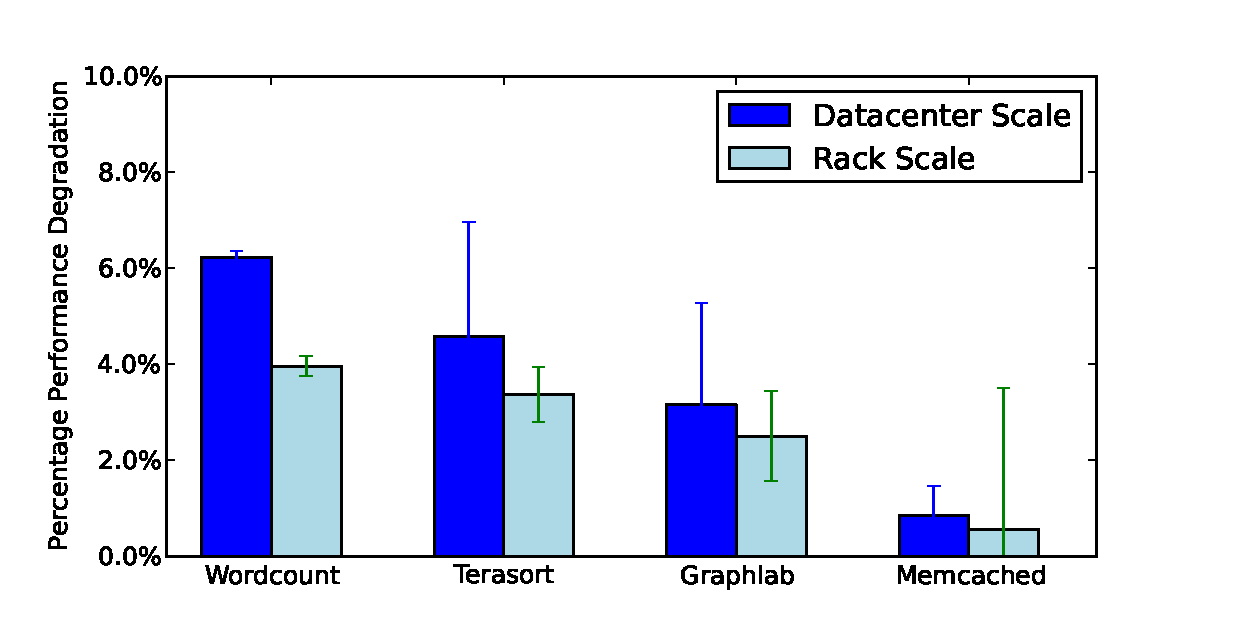
\includegraphics[width = 2.5in]{img/slowdown.eps} 
  \caption{\small{\rqc{Application layer slowdown for each of the six applications.}}}
  \label{fig:appfabric}
\end{figure}
%

%Overall, we conclude that existing protocols should be sufficient to handle disaggregated traffic.

%
% \begin{figure}
% 	\centering
% 	\begin{tikzpicture}[xscale=0.6, yscale=0.35]

% 	\draw[thick, fill=white] (-8, 5) rectangle (-5, 9); 
% 	\draw[thick, fill=white] (-8, 9.75) rectangle (-5, 11.25); 
% 	\draw[thick, fill=white] (-8, 12) rectangle (-5, 14); 
% 	\draw (-6.5, 8.5) node {\small{Network}};
% 	\draw (-6.5, 7.5) node {\small{Simulator}};
% 	\draw (-6.5, 6.5) node {\small{(Individual}};
% 	\draw (-6.5, 5.5) node {\small{Flow delays)}};
% 	\draw (-6.5, 10.5) node {\small{Scale up}};
% 	\draw (-6.5, 13.5) node {\small{Flows from}};
% 	\draw (-6.5, 12.5) node {\small{Step (a)}};
% 	\draw[thick, black, ->] (-6.5, 12) -- (-6.5, 11.25);
% 	\draw[thick, black, ->] (-6.5, 9.75) -- (-6.5, 9);
% 	\draw[thick, black, -] (-5, 7) -- (-4.5, 7);
% 	\draw[thick, black, -] (-4.5, 7) -- (-4.5, 10.5);
% 	\draw[thick, black, ->] (-4.5, 10.5) -- (-3.75, 10.5);

% 	\draw[thick, fill=white] (-3, 5) rectangle (1, 13); 
% 	\draw[thick, fill=white] (-2, 14) rectangle (0, 12); 
% 	\draw (-1, 13) node {\small{CPU}};
% 	% \draw (-1, 10.5) node {\small{Handler}};
	
% 	\draw[thick, fill=cyan] (-3.75, 9.9) rectangle (1.75, 11.1); 
% 	\draw (-1, 10.5) node {\small{SIT (Latency Injection)}};
			
% 	\draw[thick, fill=blue] (-2.75, 7.5) rectangle (-0.75, 8.5);
% 	\draw[thick, fill=green] (-2.75, 5.5) rectangle (-0.75, 7.5);
% 	\draw (-1.75, 8) node {\small{LM}};
% %	\draw (-2.75, 7.5) -- (-0.75, 7.5);
% 	\draw (-1.75, 6.5) node {\small{RM}};
% %	\draw (-2.75, 6.5) -- (-0.75, 6.5);
% %	\draw (-1.75, 6) node {\small{K$\to$O}};

% %	\draw[thick] (-0.25, 5.5) rectangle (0.75, 8.5);
% 	\draw[thick, fill=gray] (-0.25, 8.5) rectangle (0.75, 7.5);
% 	\draw[thick, fill=gray] (-0.25, 5.5) rectangle (0.75, 6.5);
% 	\draw (0.25, 7) node {\small{$\dots$}};

% 	\draw[very thick, black, dashed, <->] (-1.5, 10) -- (-1.75, 8.5);
% 	\draw[very thick, black, dashed, <->] (-0.5, 10) -- (0.25, 8.5);
% 	\draw[very thick, black, dashed, <->] (-0.5, 10) -- (-0.45, 6);

% 	\draw[very thick, black, dashed, <->] (-1.5, 11) -- (-1.5, 12);
% 	\draw[very thick, black, dashed, <->] (-0.5, 11) -- (-0.5, 12);
% 	\draw[very thick, black, dashed, <->] (-0.5, 11) -- (-0.5, 12);

% 	\end{tikzpicture}
% 	    \caption{\small{We run real-world applications on a $5$-node Amazon EC2 cluster. To emulate end-to-end network latency, we inject artificial latencies for all ``remote memory'' and ``remote disk'' accesses and measure the impact of this latency to the application-level performance. The latencies injected for each flow are now a result of network simulation results. \rc{SIT representation imprecise}}}
% 	\label{fig:system3}
% \end{figure}
